\chapter{Piattaforma Web}
\label{chp:sviluppo}
In questo capitolo è descritta la costruzione della piattaforma acquisti associata al sito divulgativo creato con {\wp}. Lo sviluppo può essere concettualmente diviso in due parti: \emph{lato server} e \emph{lato client}. Il primo si concentra sulla creazione di una base su cui interagire per tenere traccia di tutte le azioni compiute, dal flusso di acquisto, alla registrazione delle analisi, dall'aggiunta di nuovi clienti alla creazione di attestati. Il secondo invece sulle interfacce con gli utenti finali che possono essere il cliente oppure un addetto di {\fem}.

% ---------------------------------------
%          --- Lato Server ---
% ---------------------------------------
\section{Lato Server}
\label{sec:server}
Lo sviluppo della piattaforma web ha richiesto tecnologie dedicate, tra cui \emph{Django} come web framework e \emph{MySQL} per il database. In questa sezione è descritto Django e la sua configurazione fino alla realizzazione della piattaforma attraverso alcuni passaggi chiave; per approfondimenti riguardo alcune righe di codice scritte è consigliata la lettura dell'appendice~\ref{app:codice}.

\subsection{Django}
\label{subs:django}
\emph{Django} è un web framework open source per lo sviluppo di applicazioni web, scritto in linguaggio \emph{Python} e sviluppato inizialmente come progetto dalla "Django Software Foundation" (DSF), un'organizzazione indipendente senza scopo di lucro \cite{django}. È stato inizialmente concepito per gestire diversi siti di notizie, ed in seguito distribuito con una licenza BSD (Berkeley Software Distribution) nel luglio 2005.

La scelta di Django è ricaduta grazie alle sue numerose proprietà: dall'astrazione del database relazionale ad oggetti, alla
possibilità di installare funzionalità attraverso plugin, dalla robusta API per la gestione del database, al sistema di 'view generiche che evitano la stesura di codice ripetitivo per determinati casi comuni e soprattutto il sistema di template con gestore di URL basato su espressioni regolari. Django offre inoltre un efficace supporto per localizzazione, inclusa la gestione di traduzioni in molte lingue dell'interfaccia amministrativa.

\subsection{Configurazione}
\label{subs:config}
Il primo passo è stato l'installazione delle componenti di Django attraverso la creazione del progetto (nome di esempio \texttt{mysite}), con il comando da terminale:
\begin{verbatim}
$ django-admin startproject mysite
\end{verbatim}

così da ottenere la seguente configurazione di file:
\begin{small}
\begin{verbatim}
mysite/
    manage.py
    mysite/
        __init__.py
        settings.py
        urls.py
        wsgi.py
\end{verbatim}
\end{small}

Abbiamo quindi impostato nel file \texttt{settings.py} il database scelto, le lingue del sistema, il percorso dei file statici, dei media e le \texttt{INSTALLED\_APPS}.

Le \texttt{INSTALLED\_APPS} sono una sorta di librerie usate per l'aggiunta di componenti al progetto costruito; le più importanti sono:
\begin{itemize}
 \item \texttt{django.contrib.admin} - il creatore automatico del pannello admin
 \item \texttt{django.contrib.auth} - il sistema di autenticazione
 \item \texttt{django.contrib.sessions} - il framework per il controllo delle sessioni
 \item \texttt{django.contrib.messages} - il framework di controllo per i messaggi
 \item \texttt{django.contrib.staticfiles} - il gestore dei file statici
\end{itemize}

\subsection{Costruzione}
\label{subs:crea}
Durante tutta la fase di sviluppo è stato necessario avviare il \emph{development server} attraverso il comando da terminale:
\begin{verbatim}
$ python manage.py runserver
\end{verbatim}
per simulare il comportamento del server in modo da generare il sito all'indirizzo \texttt{http://127.0.0.1:8000/}

Una componente fondamentale è rappresentata dai \emph{modelli}, strutture associabili concettualmente alle classi in Java; in funzione alle richieste avanzate da {\fem} il diagramma in figura~\ref{fig:modelli} rappresenta come sono stati configurati i modelli con i relativi attributi.

\begin{figure}
 \centering
 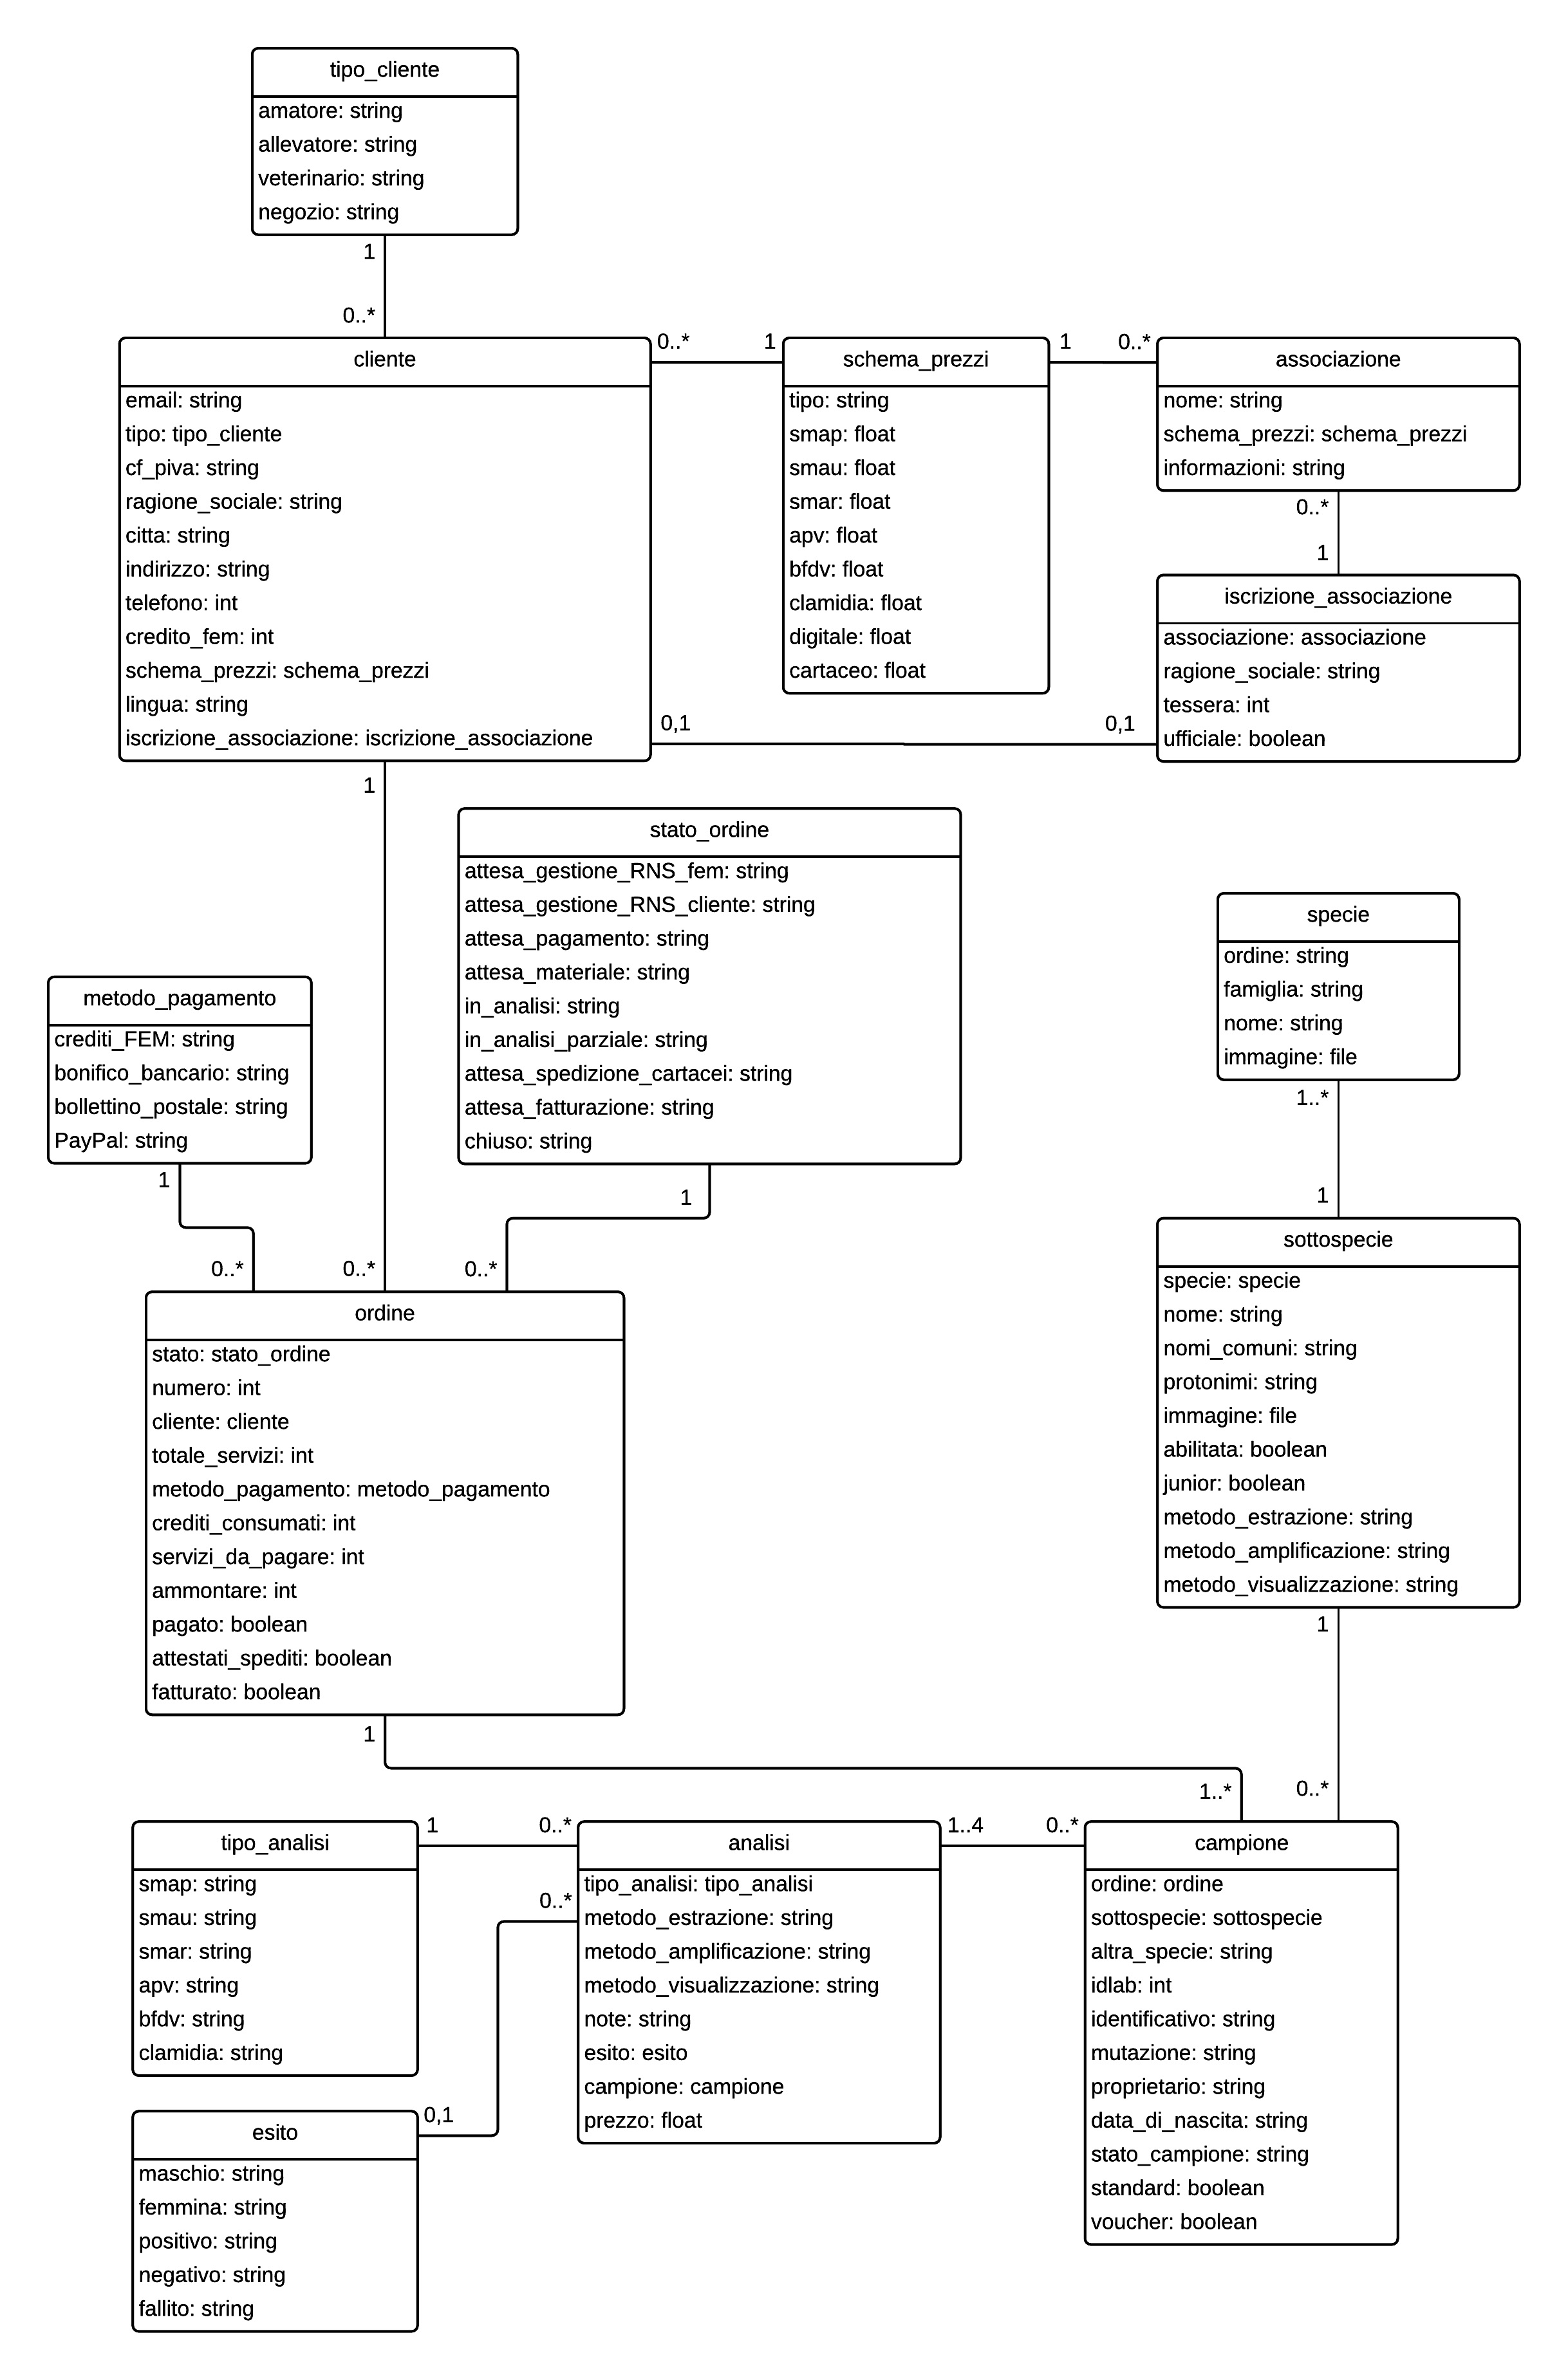
\includegraphics[width=0.85\textwidth]{images/modelli} 
 \caption{configurazione modelli}
 \label{fig:modelli}
\end{figure}

Nei seguenti paragrafi sono descritti i principali modelli.

\subsection*{clienti.py}
\label{subs:clienti}
Il cliente è un componente delicato ed importante del sistema; 

È identificato univocamente dall'indirizzo \texttt{email} inserito al momento della registrazione e ha l'attributo \texttt{ragione\_sociale} per indicare nome e cognome in caso di privato. L'attributo \texttt{tipo} è necessario in quanto per {\fem} il cliente può essere differenziato in quattro tipi: Amatore, Allevatore, Veterinario e Negozio. Ogni cliente ha altri numerosi attributi per ogni dato personale relativo all'indirizzo (necessario per la spedizione degli attestati generati al termine delle analisi), contatti telefonici e \texttt{lingua\_preferita} per tradurre il sistema correttamente.

La possibilità di ogni cliente di acquistare pacchetti di \emph{Crediti FEM} (cioè una somma di denaro pronta per gli acquisti pagata anticipatamente, in modo da non dover effettuare il pagamento al termine di ogni ordine) ha reso necessario indicare la quantità di crediti posseduta da ogni cliente in un apposito attributo.

Inoltre ogni cliente può essere iscritto ad una associazione convenzionata all'azienda {\fem} e deve poter inserire il proprio numero di tessera per accedere agli sconti relativi; per farlo si deve dare uno sguardo ai modelli \texttt{associazioni.py} e \texttt{prezzi.py}.

\subsection*{prezzi.py}
\label{subs:prezzi}
Ogni \texttt{SchemaPrezzi} è identificato dal \texttt{nome} e può essere associato a nessuno, uno o tanti clienti. Esso definisce i costi fissi delle commissioni per ogni metodo di pagamento scelto, il prezzo degli attestati e il prezzo di ogni analisi, che tendenzialmente può variare tra uno schema prezzo e l'altro.

In particolare abbiamo deciso di differenziare gli schemi prezzi secondo una caratteristica principale: schema \emph{Pacchetti} o \emph{Convenzioni}.

Uno schema prezzi del tipo \emph{Pacchetti} è caratteristico di un cliente standard, che può usufruire di sconti vincolati a quantità, ad esempio con l'acquisto di un analisi APV associato ad un analisi SMAP riduce il costo di entrambe. Uno schema prezzi del tipo \emph{Convenzioni} invece è adatto per i clienti che risultano iscritti ad una associazione che ha attivato una convenzione con {\fem}; questo tipo di schema prezzi modifica il costo di tutte o alcune analisi anche in relazione alle specie del campione scelta.

\subsection*{associazioni.py}
\label{subs:associazioni}
Una \texttt{Associazione} è caratterizzata da un nome e da uno schema prezzi associato. \texttt{IscrizioneAssociazione} indica la correlazione tra un cliente, indicato attraverso nome e numero di tessera, e una associazione. È stato aggiunto anche l'attributo booleano \texttt{ufficiale} per indicare quando l'iscrizione di un cliente ad una associazione è verificata, in quanto gli elenchi degli associati sono forniti dalle associazioni stesse a {\fem} e non integrati nel sistema.

\subsection*{ordini.py}
\label{subs:ordini}
L'\texttt{Ordine} è il componente più delicato e complesso del sistema a causa del suo flusso rappresentato in figura~\ref{fig:flusso-ordine}.

\begin{figure}
 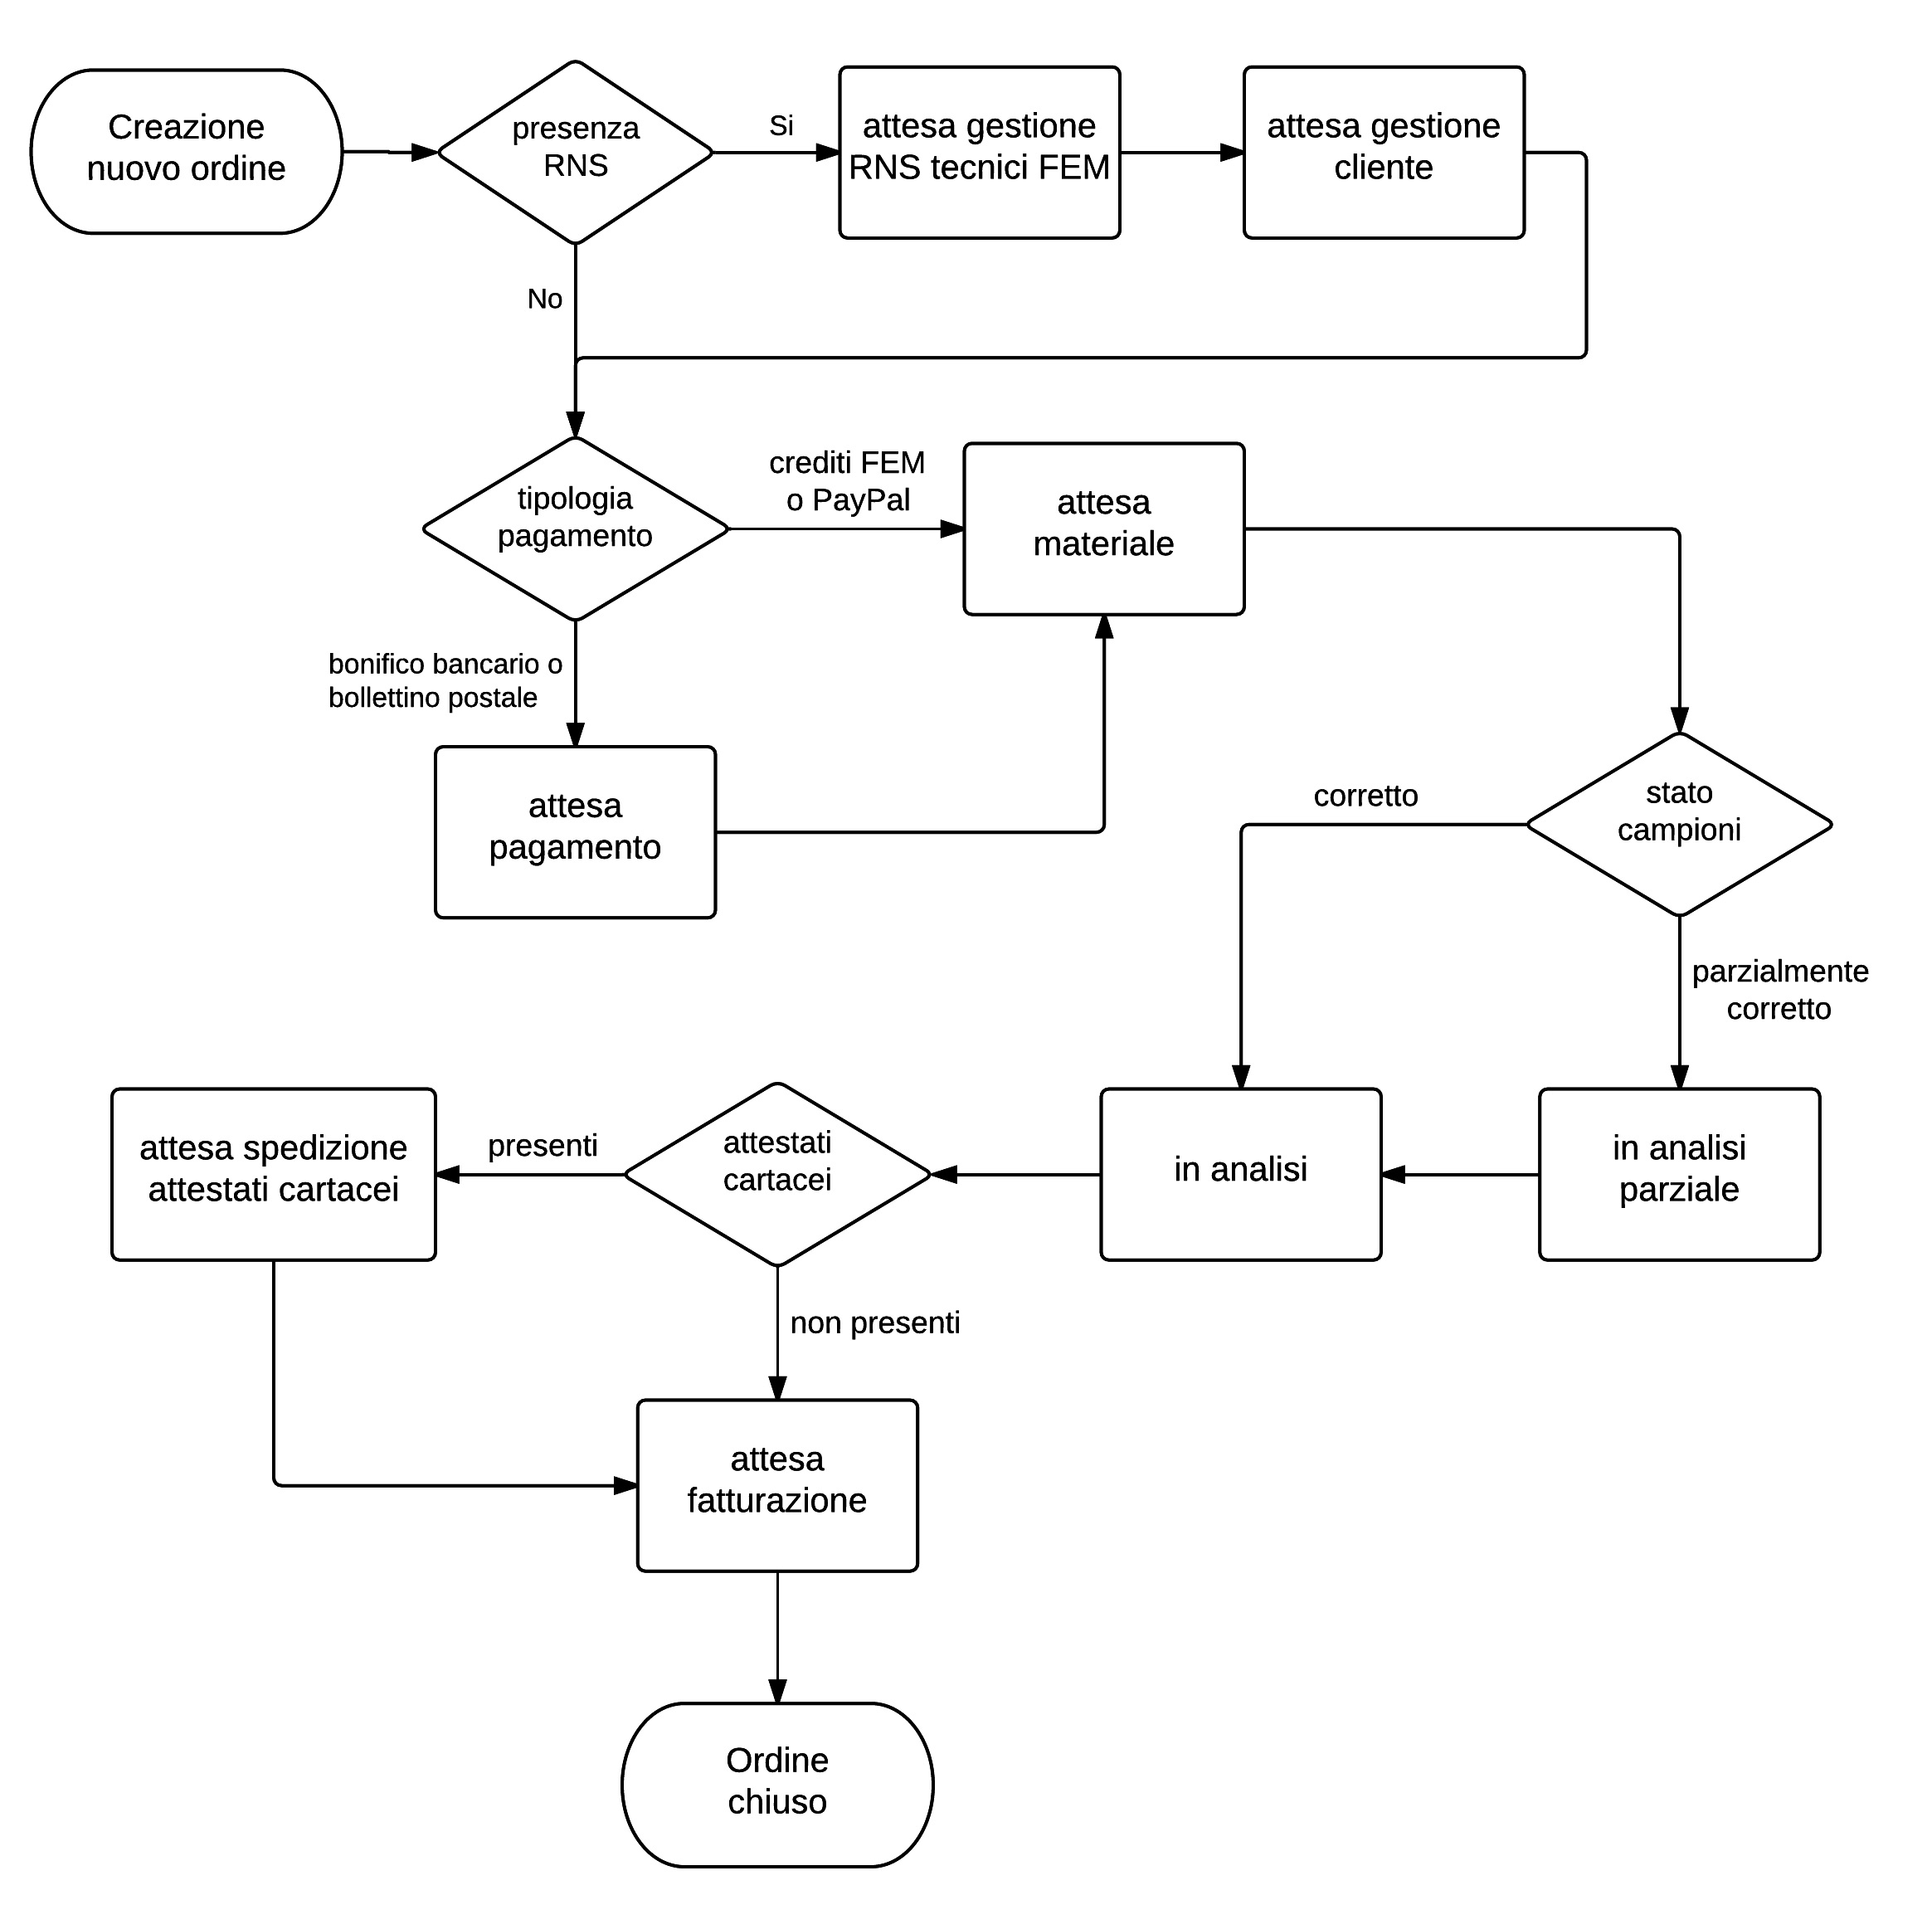
\includegraphics[width=1\textwidth]{images/flusso-ordine} 
 \caption{flusso ordine}
 \label{fig:flusso-ordine}
\end{figure}

Esso è caratterizzato dal \texttt{cliente} che l'ha creato, dall'attributo \texttt{stato} che indica in quale posizione del flusso si trova e univocamente dal \texttt{numero}.
Altri attributi interessanti sono:
\begin{itemize}
 \item \texttt{metodo\_pagamento} indica il metodo di pagamento scelto tra le possibilità offerte da {\fem}
 \item \texttt{totale\_servizi} indica il costo delle analisi richieste con aggiunte le eventuali spese di spedizione per gli attestati cartacei 
 \item \texttt{crediti\_consumati} indica la quantità di crediti FEM utilizzati per pagare l'ordine
 \item \texttt{servizi\_da\_pagare} indica il \texttt{totale\_servizi} da cui sono stati sottratti i \texttt{crediti\_consumati}
 \item \texttt{ammontare} indica il \texttt{totale\_servizi} sommato all'eventuale costo di commissione previsto dal metodo di pagamento
\end{itemize}

Per aiutare la gestione del flusso sono utilizzati i booleani \texttt{pagato}, \texttt{fatturato} e \texttt{attestati\_spediti} che indicano rispettivamente se l'ordine è stato pagato, fatturato e se sono stati inviati gli attestati cartacei richiesti al cliente.

\subsection*{specie.py}
\label{subs:specie}

Per descrivere il modello relativo le specie è necessario prima di tutto spiegare che la tassonomia (dal greco \emph{taxis} 'ordinamento', e \emph{nomos} 'norma') è definita in generale come la disciplina della classificazione. Abitualmente si impiega il termine per indicare la tassonomia biologica, ossia la disciplina scientifica che si occupa di attribuire un nome agli organismi viventi e di classificarli. La gerarchia di classificazione biologica secondo gli otto principali ranghi tassonomici è descritta in figura~\ref{fig:tassonomia} (le posizioni intermedie della classifica non sono mostrate in figura).

\begin{figure}
 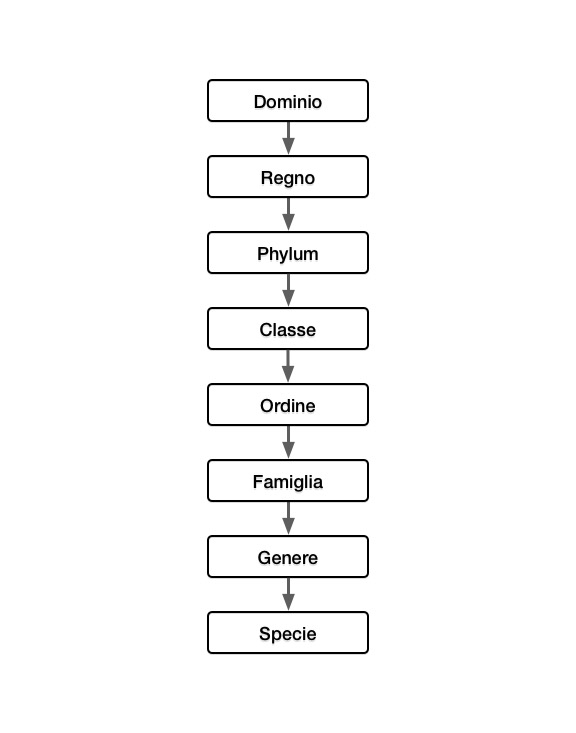
\includegraphics[width=1\textwidth]{images/tassonomia} 
 \caption{Classificazione biologica secondo i principali ranghi tassonomici}
 \label{fig:tassonomia}
\end{figure}

Il Portale Avifauna si occupa di analisi su un complesso di uccelli che vivono in una determinata regione, ma non tutti gli esemplari richiedono lo stesso tipo di approccio o tecnica per effettuare la medesima analisi. La differenziazione principale scelta è quindi in base a \emph{specie} e \emph{sottospecie}.

Il modello \texttt{specie.py} si occupa di creare la base per questa differenziazione. 

Ogni specie ha \texttt{ordine}, \texttt{famiglia}, \texttt{nome} e un \texttt{immagine} per descriverla; ogni \texttt{sottospecie} ha a sua volta la \texttt{specie} di riferimento, \texttt{nome}, \texttt{immagine} ed eventuali \texttt{nomi\_comuni} e \texttt{protonimi}. 

Le sottospecie sono anche caratterizzate dalla proprietà \texttt{junior} ovvero considerate \emph{giovani} perché {\fem} non ha ancora acquisito un numero soddisfacente di dati relativi alla sottospecie in questione, quindi non garantisce al 100\% il corretto risultato delle analisi di tipo sessaggio effettuate. 

Per facilitare il lavoro in laboratorio sono stati creati anche gli attributi testuali \texttt{metodo\_estrazione},  \texttt{metodo\_amplificazione} e \texttt{metodo\_visualizzazione} utili agli addetti per riconoscere più rapidamente quali tecniche applicare e come eseguire le operazioni di analisi.

\subsection*{campioni.py}
\label{subs:campioni}
Analogamente ad un qualsiasi servizio di vendita o e-commerce, ogni ordine è una raccolta di uno o più oggetti; nel Portale Avifauna gli oggetti sono i \texttt{campioni}, ovvero i soggetti su cui sono richieste le analisi da effettuare.

Ogni campione ha i seguenti attributi:
\begin{itemize}
 \item \texttt{ordine} per indicare il numero di ordine di riferimento
 \item \texttt{identificativo} ovvero il nome dell'esemplare o il codice RNA+Anello
 \item \texttt{specie} o un eventuale \texttt{altra\_specie} in caso in cui non sia presente nell'elenco fornito da {\fem}
 \item \texttt{mutazione}, \texttt{proprietario} e \texttt{data\_di\_nascita} utili soprattutto per la generazione degli attestati
 \item \texttt{idlab}, \texttt{stato\_campione}, \texttt{standard} e \texttt{voucher} utili per il lavoro in laboratorio
\end{itemize} 

Il campo \texttt{identificativo} segue le regole fornite dalla \emph{Federazione Ornicoltori Italiani} (F.O.I.), un ente che raggruppa tutti gli appassionati ornicoltori e gli allevatori di uccelli con lo scopo di promuovere lo studio, il miglioramento, lo sviluppo e la conservazione del patrimonio ornitologico \cite{foi}. La F.O.I. ha regolamentato che per poter partecipare alle Manifestazioni Ornitologiche occorre che gli uccelli abbiano alla propria zampa un anellino in modo da riportare i dati dell'allevatore (mediante la sigla \emph{R.N.A.}), l'anno di nascita del soggetto e un numero progressivo, attraverso il quale è possibile risalire ai genitori contattando l'allevatore che avrà avuto cura di registrare i dati genealogici in appositi registri. Il campo identificativo indicherà quindi il nome dell'esemplare in caso di privati e RNA+Anello in caso di allevatori professionisti.

Per facilitare il lavoro in laboratorio sono stati introdotti gli attributi \texttt{idlab} che indica il numero progressivo e univoco utilizzato in laboratorio e \texttt{stato\_campione} per indicare eventuali caratteristiche del campione, il quale può essere normale, mancante, inadatto, rischioso o annullato. 

Il flusso dell'ordine può subire variazioni in funzione degli stati dei propri campioni; ad esempio se uno é mancante, inadatto o rischioso il cliente viene tempestivamente contattato da un dipendente di {\fem} in modo da decidere come comportarsi. In caso di campione mancante o inadatto il cliente può decidere di annullarlo e proseguire l'ordine oppure inviare di nuovo le piume del soggetto.

Altri attributi interessanti sono \texttt{voucher}, che funge da 'etichetta' per evidenziare un campione che viene preso di riferimento per future analisi, e soprattutto \texttt{standard}.

Una specie, come spiegato precedentemente in nel paragrafo dedicato, può essere definita \emph{junior} in caso in cui {\fem} lo reputi necessario in quanto non ha ancora eseguito un numero minimo di analisi di tipo sessaggio su di essa per sentirsi fiduciosa da assicurare il successo delle analisi. Per questo motivo, al momento della creazione dell'ordine, nel caso in cui venga aggiunto un campione di specie junior, si chiede di aggiungere eventuali campioni (se il cliente ne è in possesso) definiti \emph{standard}, ovvero esemplari di cui il cliente è già a conoscenza del sesso (tipicamente i genitori) in modo da fornire ai tecnici di laboratorio di {\fem} maggior materiale di riferimento ed aumentare così le possibilità di successo delle analisi.

Su ciascun \texttt{campione} possono essere eseguite una o più \emph{analisi} con il vincolo di non richiedere più di una analisi di tipo sessaggio per ognuno (per maggiori dettagli si guardi il paragrafo dedicato alle analisi).

\subsection*{analisi.py}
\label{subs:analisi}
Ad oggi {\fem} è in grado di offrire servizi di analisi di tipo \emph{Sessaggio molecolare} (determinazione di genere maschio o femmina) e \emph{identificazione di patologie}.

I primi sono suddivisi in:
\begin{itemize}
 \item \textbf{SMAP, Sessaggio Molecolare di Avifauna da Piuma}: analisi del DNA a partire da piume per stabilire il sesso del soggetto.
 \item \textbf{SMAU, Sessaggio Molecolare di Avifauna da Uovo}: analisi del DNA a partire da frammenti di uovo.
 \item \textbf{SMAR, Sessaggio Molecolare di Avifauna Rapido}: analisi rapida del DNA a partire da piume.
\end{itemize}

I secondi in:
\begin{itemize}
 \item \textbf{APV-Avian Polioma Virus}: un agente patogeno virale diffuso in tutto il mondo in grado di infettare un ampio spettro di uccelli; poichè gli adulti solitamente sono portatori asintomatici, sono i principali responsabili della persistenza, della trasmissione e della diffusione della malattia. {\fem} esegue analisi di screening di APV attraverso PCR (Polymerase Chain Reaction) a partire da piume e/o da prelievo ematico.
 \item \textbf{BFDV Circovirus}: virus che attacca i tessuti di becco, piume e artigli causando progressive malformazioni fino alla necrosi. Le analisi vengono eseguite attraverso PCR a partire da piume.
 \item \textbf{Clamidia - Chlamydophila psittaci}: un batterio che si può trovare nel torrente circolatorio, nei tessuti, negli escrementi e nelle piume degli uccelli.
\end{itemize}

Le analisi sono quindi caratterizzate dal \texttt{tipo\_analisi} tra quelli elencati precedentemente e dal \texttt{campione} di riferimento il quale influenza i metodi di estrazione, amplificazione e visualizzazione consigliati in funzione della specie.

Hanno anche un campo dedicato all'\texttt{esito} (di tipo Maschio, Femmina o Fallito nel caso di analisi di sessaggio; Positivo, Negativo o Fallito in caso di identificazione di patogeno) e le variabili booleane per indicare se è stato richiesto \texttt{attestato\_cartaceo} o \texttt{attestato\_digitale}. Ogni analisi ha inoltre un \texttt{prezzo} definito in base allo schema prezzi applicato.

% ---------------------------------------
%           --- Lato Client ---
% ---------------------------------------
\newpage
\section{Lato Client}
\label{sec:client}
La struttura alla base della piattaforma web per il Portale Avifauna può essere rappresentata attraverso la divisione dei modelli descritta in precedenza (figura~\ref{fig:modelli}),mentre di seguito sono descritte le tecnologie utilizzate per la costruzione dell'interfaccia utente, ovvero: \emph{HTML}, \emph{CSS}, \emph{\js} e \emph{Bootstrap} (paragrafo~\ref{subs:strumenti}).

Interfaccia utente costruita sia per il cliente finale (paragrafo~\ref{subs:cliente}) che per i tecnici di {\fem} che lavorano tutti i giorni con il sistema (paragrafo~\ref{subs:admin}); per ulteriori approfondimenti sull'utilizzo sono disponibili rispettivamente le appendici~\ref{app:cliente} e ~\ref{app:admin}.

\subsection{Strumenti utilizzati}
\label{subs:strumenti}

\subsection*{HTML}
\label{subs:html}
\emph{HTML} (HyperText Markup Language) è il linguaggio di markup utilizzato per la formattazione e impaginazione di documenti ipertestuali disponibili nel World Wide Web sotto forma di pagine web. È un linguaggio di pubblico dominio, la cui sintassi è stabilita dal World Wide Web Consortium (W3C) \cite{html} ed è utilizzato per descrivere le modalità di impaginazione o visualizzazione grafica (layout) del contenuto, testuale e non, di una pagina web attraverso tag di formattazione.

HTML è stato sviluppato verso la fine degli anni ottanta da Tim Berners-Lee al CERN di Ginevra insieme al protocollo HTTP dedicato al trasferimento di documenti in tale formato. Negli anni novanta il linguaggio ha avuto una forte diffusione in seguito ai primi utilizzi commerciali del web e attualmente i documenti HTML sono in grado di incorporare molte tecnologie che offrono la possibilità di aggiungere al documento ipertestuale controlli più sofisticati sulla resa grafica, interazioni dinamiche con l'utente, animazioni interattive e contenuti multimediali. Si tratta di linguaggi come CSS, JavaScript e jQuery.

Il componente principale della sintassi di questo linguaggio è l'elemento inteso come struttura di base a cui è delegata la funzione di formattare i dati o indicare al browser delle informazioni; ogni elemento è racchiuso all'interno di marcature dette tag, costituite da una sequenza di caratteri racchiusa tra due parentesi angolari o uncinate ($< >$).

L'ultima versione è detta \emph{HTML5}, pubblicata come W3C Recommendation da ottobre 2014. Le novità introdotte con HTML5 sono finalizzate soprattutto a migliorare il disaccoppiamento fra struttura (definita dal markup) e contenuti di una pagina web.

\subsection*{CSS}
\label{subs:css}
\emph{CSS} (Cascading Style Sheets) è un linguaggio usato per definire la formattazione di documenti HTML, XHTML e XML. Le regole per comporre il CSS sono contenute, come per HTML, in un insieme di direttive dette W3C Recommendations emanate a partire dal 1996 dal consorzio stesso \cite{css}.

L'introduzione del CSS si è resa necessaria a partire dalla metà degli anni novanta per separare i contenuti dalla formattazione e permettere una programmazione più chiara e facile da utilizzare, sia per gli autori delle pagine HTML che per gli utenti ed ha raggiunto l'ultima versione (definita \emph{CSS3}) in completo equilibrio con HTML5.

\subsection*{JavaScript}
\label{subs:js}
\emph{{\js}} è un linguaggio di scripting orientato agli oggetti e agli eventi, comunemente utilizzato nella programmazione web lato client per la creazione, in siti ed applicazioni web, di effetti dinamici interattivi tramite funzioni di script. 

È stato originariamente sviluppato da Brendan Eich della Netscape Communications con il nome di Mocha e successivamente di LiveScript, solo in seguito è stato rinominato {\js}; è stato standardizzato per la prima volta nella fine degli anni novanta con il nome \emph{ECMAScript} e l'ultimo standard, di giugno 2015, è ECMA-262 Edition 6 \cite{jsecma}.

Una delle caratteristiche principali di {\js} è di essere un linguaggio interpretato: in {\js} lato client l'interprete è incluso nel browser che si sta utilizzando il quale, quando viene visitata una pagina web che contiene il codice di uno script {\js}, porta in memoria primaria lo script e lo esegue. Le interfacce che consentono a {\js} di rapportarsi con un browser sono chiamate DOM (Document Object Model). 

Molti siti web usano la tecnologia {\js} lato client per creare potenti applicazioni web dinamiche.

\subsection*{Bootstrap}
\label{subs:bootstrap}
\emph{{\b}} è un framework che raccoglie strumenti liberi per la creazione di siti e applicazioni per il web, tra cui modelli basati su HTML, CSS e {\js} per il controllo di struttura, tipografia e interfaccia \cite{bootstrap}.

{\b} è stato sviluppato da Mark Otto e Jacob Thornton a Twitter come un framework per uniformare i diversi componenti utilizzati fino a quel momento ed è stato rilasciato nell'agosto 2011 come progetto open source.

{\b} è compatibile con le ultime versioni di tutti i principali browser e dalla versione 2.0 supporta anche il responsive web design, ovvero una serie di tecniche per adattarsi graficamente in modo automatico al dispositivo con il quale viene visualizzata la pagina web, sempre più vitale in un mondo dove l'utilizzo di dispositivi mobili come tablet e smartphone è in costante crescita. Ad oggi l'ultima versione è la 3.3.5 di maggio 2015, ma è già in fase di sviluppo la 4.0 \cite{bootstrap-github}.

Associato a {\b} è stato utilizzato anche \emph{Font Awesome}, un toolkit di font e icone basato su CSS, creato da Dave Gandy per l'utilizzo in Twitter Bootstrap \cite{fontawesome} \cite{fontawesome-github}. Esso permette una maggiore personalizzazione di icone e tipografia molto utile nella Piattaforma Avifauna per comunicare graficamente con il cliente graficamente in modo immediato.

\newpage
\subsection{Vista Cliente}
\label{subs:cliente}
Il cliente finale può compiere le azioni rappresentate nella figura~\ref{fig:flusso-cliente}.

Il cliente si può dividere in due categorie: \emph{registrato} e \emph{non registrato}. Per registrarsi al sistema è sufficiente seguire l'apposita procedura, dopodiché effettuando il login si accede alla propria pagina personale, dove si possono modificare i propri dati personali, acquistare pacchetti di crediti FEM, ma soprattutto monitorare i propri ordini e crearne di nuovi. 

Queste azioni sono descritte meglio nell'appendice~\ref{app:cliente} e devono essere supportate da un adeguata interfaccia; per farlo sono stati utilizzati tutti gli strumenti descritti in precedenza.

Ogni schermata visualizzata dal cliente è una pagina HTML generata dalla piattaforma sottostante, ovvero Django il quale ha bisogno di una gestione dinamica dei file HTML e l'approccio ottimale è l'utilizzo dei \emph{templates}.
Un template contiene porzioni statiche del codice HTML desiderato e permette la riproduzione di alcune o intere porzioni di codice in altri file per evitare inutili dupicati.

\begin{figure}
 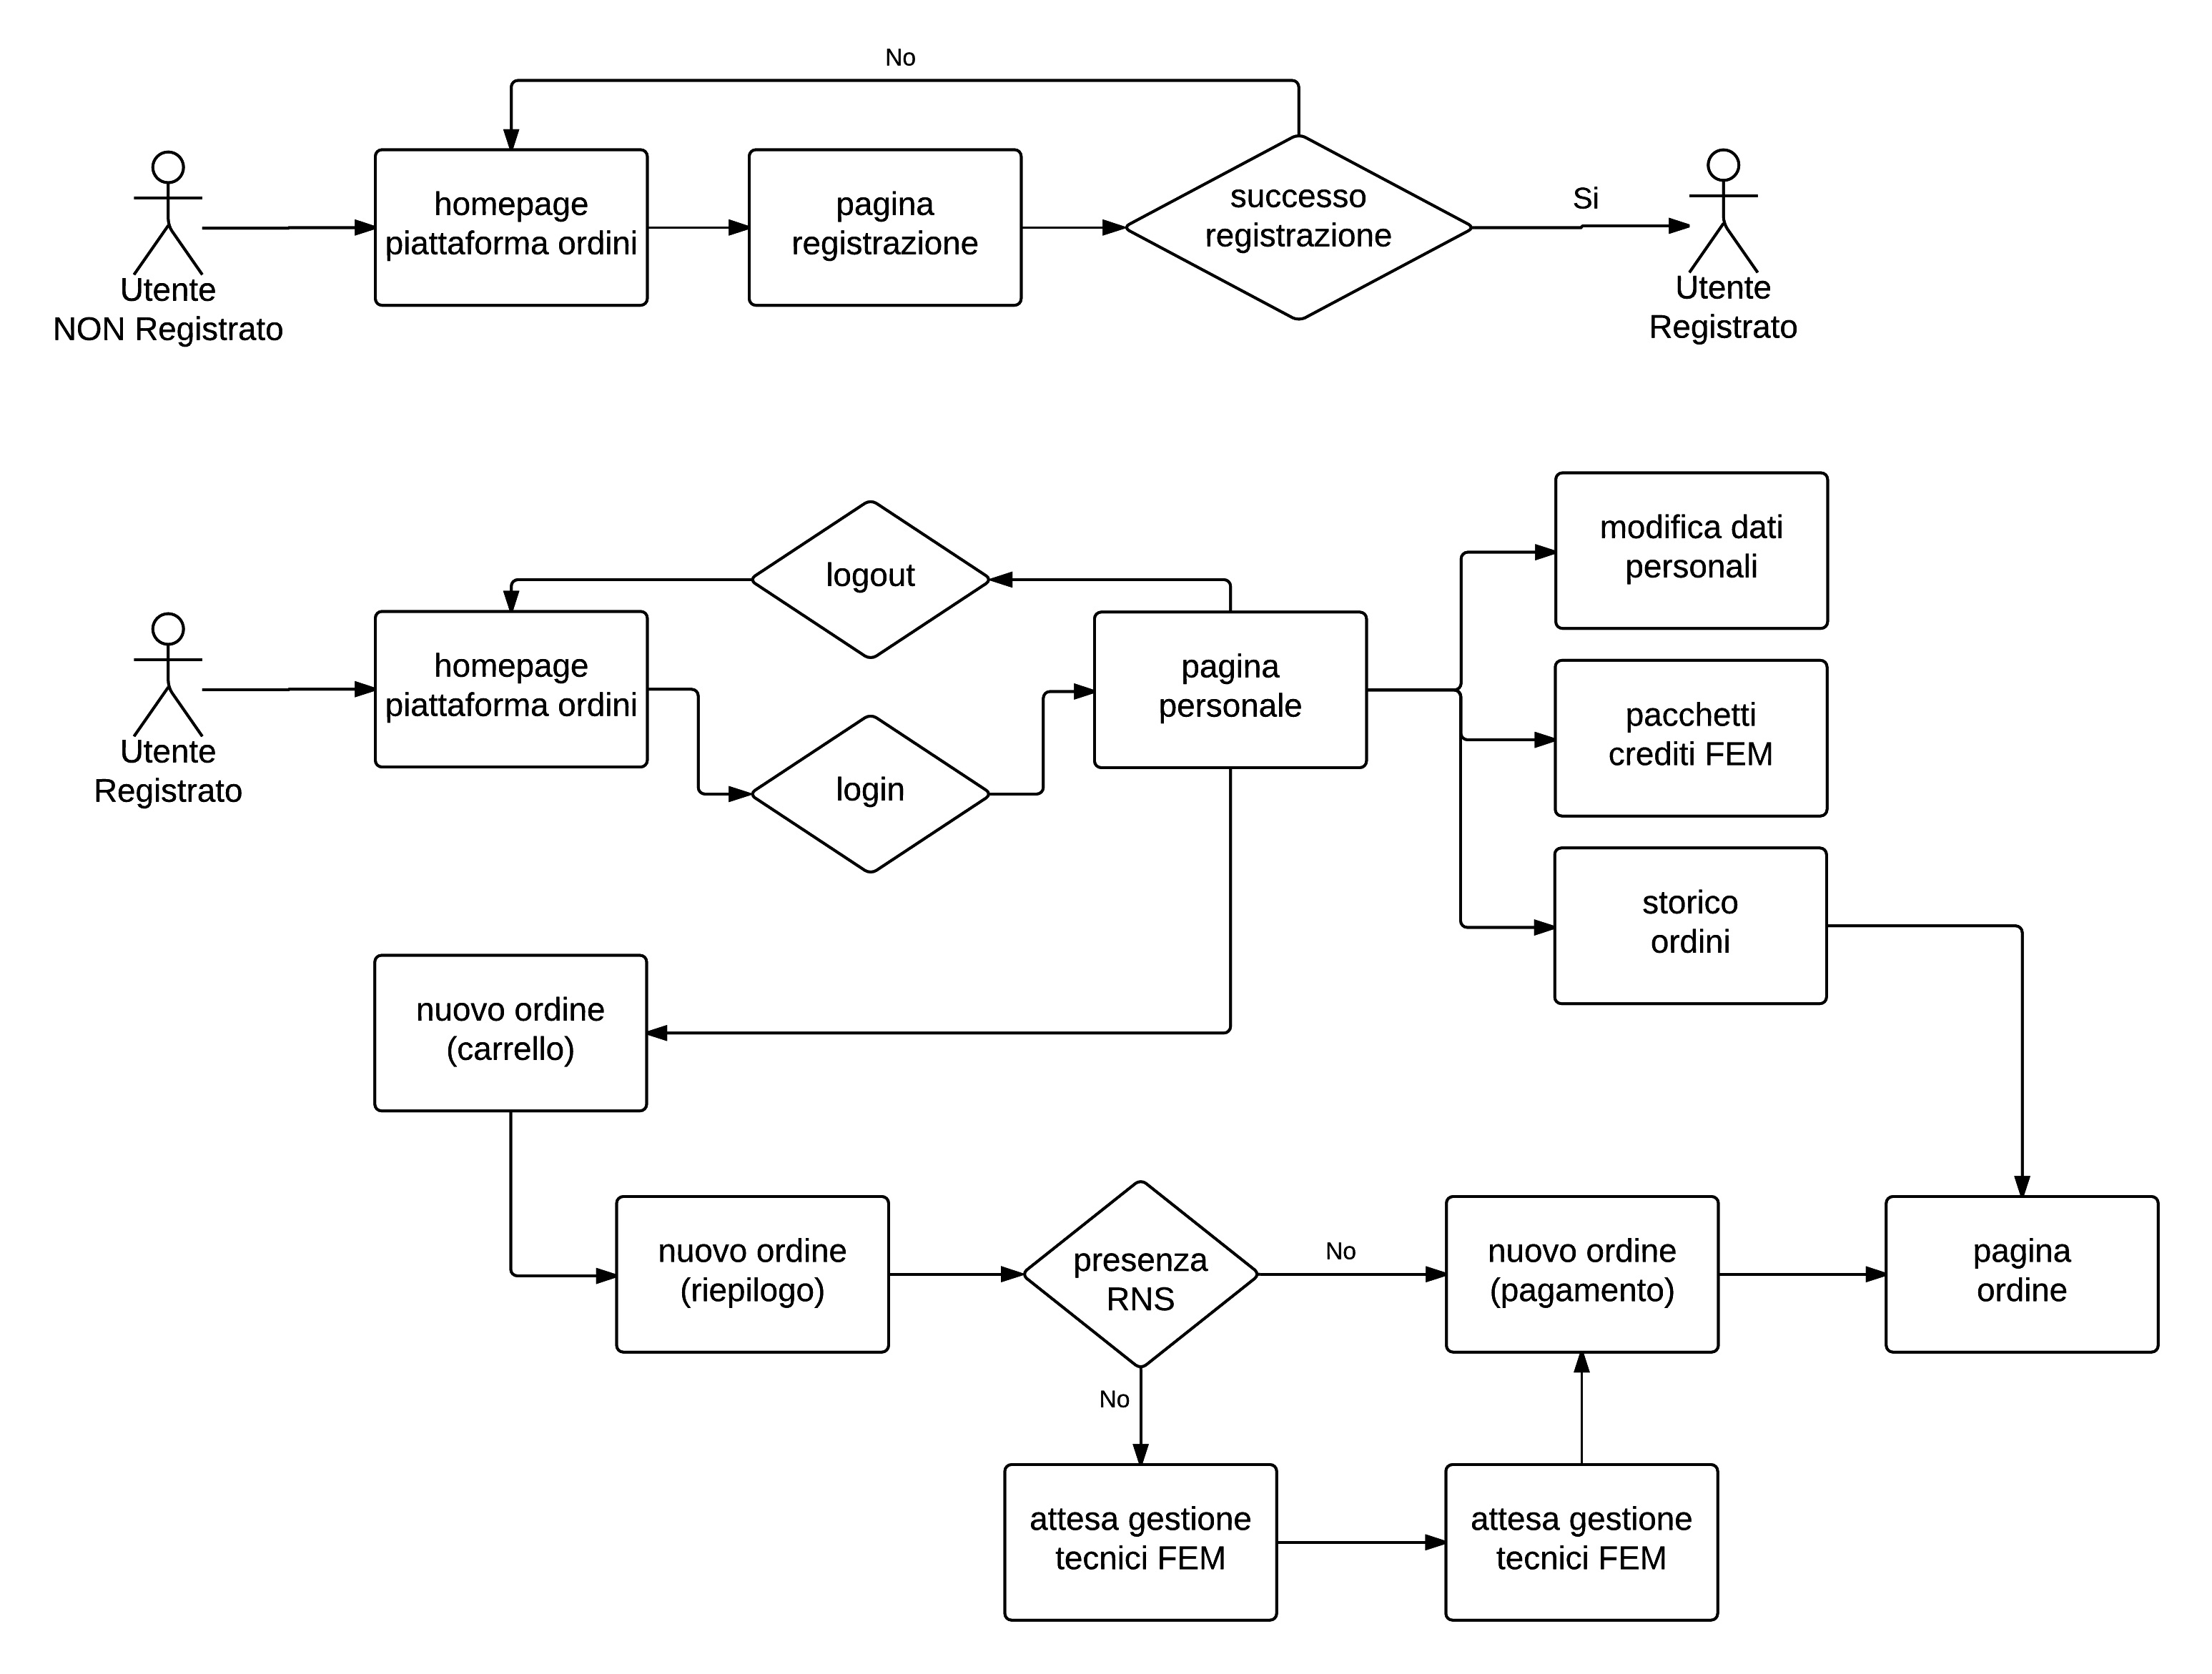
\includegraphics[width=1\textwidth]{images/flusso-cliente} 
 \caption{flusso cliente}
 \label{fig:flusso-cliente}
\end{figure}

Sono stati quindi sfruttati alcuni comandi:
\begin{itemize}
 \item per includere un file HTML all'interno di un altro
  \begin{verbatim} 
    
  \end{verbatim}
 \item per indicare un blocco di contenuto specifico, ad esempio inserendo \texttt{jsexec} al posto di \dots si indica una porzione dedicata a script {\js}, o ancora, scrivendo \texttt{title} si indica il titolo della pagina.
  \begin{verbatim} 
    
  \end{verbatim}
 \item per descrivere come il file richieda di essere una estensione di un altro (molto utile per creare e modificare lo stile di base di tutti i file generati in uno unico, in questo progetto chiamato \texttt{base.html}).
  \begin{verbatim} 
    
  \end{verbatim} 
\end{itemize}
Alcuni esempi di utilizzo sono mostrati nell'appendice~\ref{app:codice}.

Con la creazione del file \texttt{base.html} è stato possibile definiti i file statici CSS e {\js} utilizzati in tutte le pagine una sola volta, senza ripetizioni, generando uno stile solido che permette però personalizzazioni centralizzate.

Dalla figura~\ref{fig:flusso-cliente} del flusso cliente si evince come il primo passo sia stato costruire una sorta di homepage o schermata principale per introdurre i clienti non registrati al Portale (file chiamato \texttt{home.html}) e da qui, attraverso la barra di navigazione, dare la possibilità di effettuare il login o la registrazione.

\subsection*{Registrazione e pagina personale}
\label{subs:preg-ppers}
La pagina di registrazione (\texttt{register.html}) ha richiesto l'utilizzo di codice {\js} principalmente per il controllo dei dati inseriti nei campi del form, in particolare il controllo in browser della compilazione di tutti i campi obbligatori e della loro correttezza sintattica in modo da evitare inutili comunicazioni con il server che porterebbero a una, seppur lieve, perdita di tempo.

I controlli sono dei semplici 'validatori' che assegnano \texttt{true} alla variabile \texttt{any\_error} in modo da visualizzare un messaggio di errore al momento dell'invio del form. Per rendere ancora più esplicito il messaggio di errore è stato inserito in un \emph{modale}, strumento introdotto da {\b} che consiste in un \tag{div} al centro della viewport (ovvero la regione di pagina che viene visualizzata nel monitor) che monopolizza l'attenzione. All'interno di esso viene inserito il testo relativo all'errore. Ad esempio
\begin{verbatim}
if(any_error) {
 modal
  .body("Sono presenti alcuni errori")
}
\end{verbatim}

Una volta completato il processo di registrazione il cliente visualizza la propria pagina personale (schema in figura~\ref{fig:pagina-personale-s}) in cui può controllare la propria cronologia di ordini, modificare i dati personali, acquistare pacchetti crediti FEM, ma soprattutto creare un nuovo ordine.

\begin{figure}
 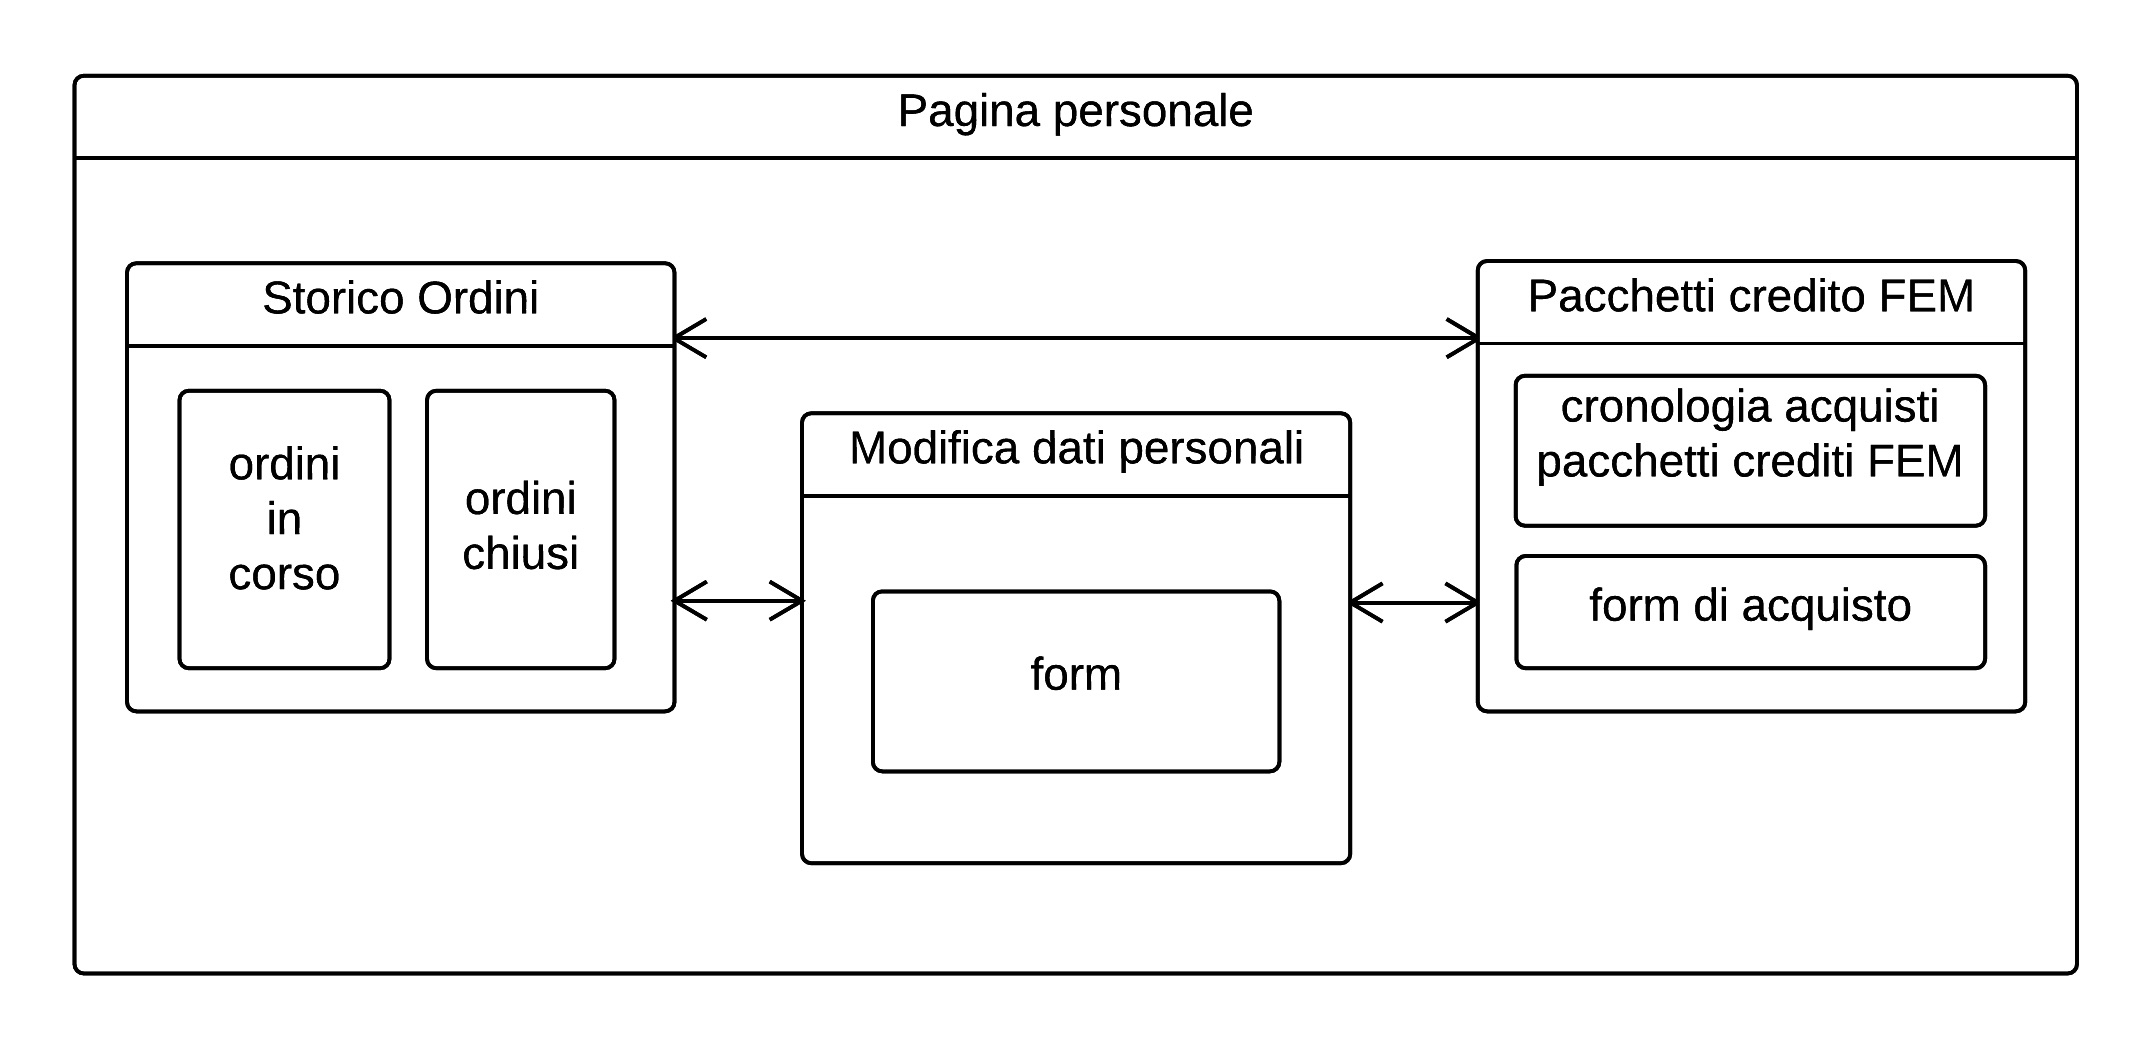
\includegraphics[width=1\textwidth]{images/pagina-personale-s} 
 \caption{pagina personale}
 \label{fig:pagina-personale-s}
\end{figure}

\subsection*{Nuovo ordine}
\label{subs:pno}
La pagina di creazione dell'ordine, descritta in figura~\ref{fig:nuovo-ordine-s}, è divisa in tre blocchi come sono le sue fasi: \emph{carrello}, \emph{riepilogo} e \emph{pagamento}.

\begin{figure}
 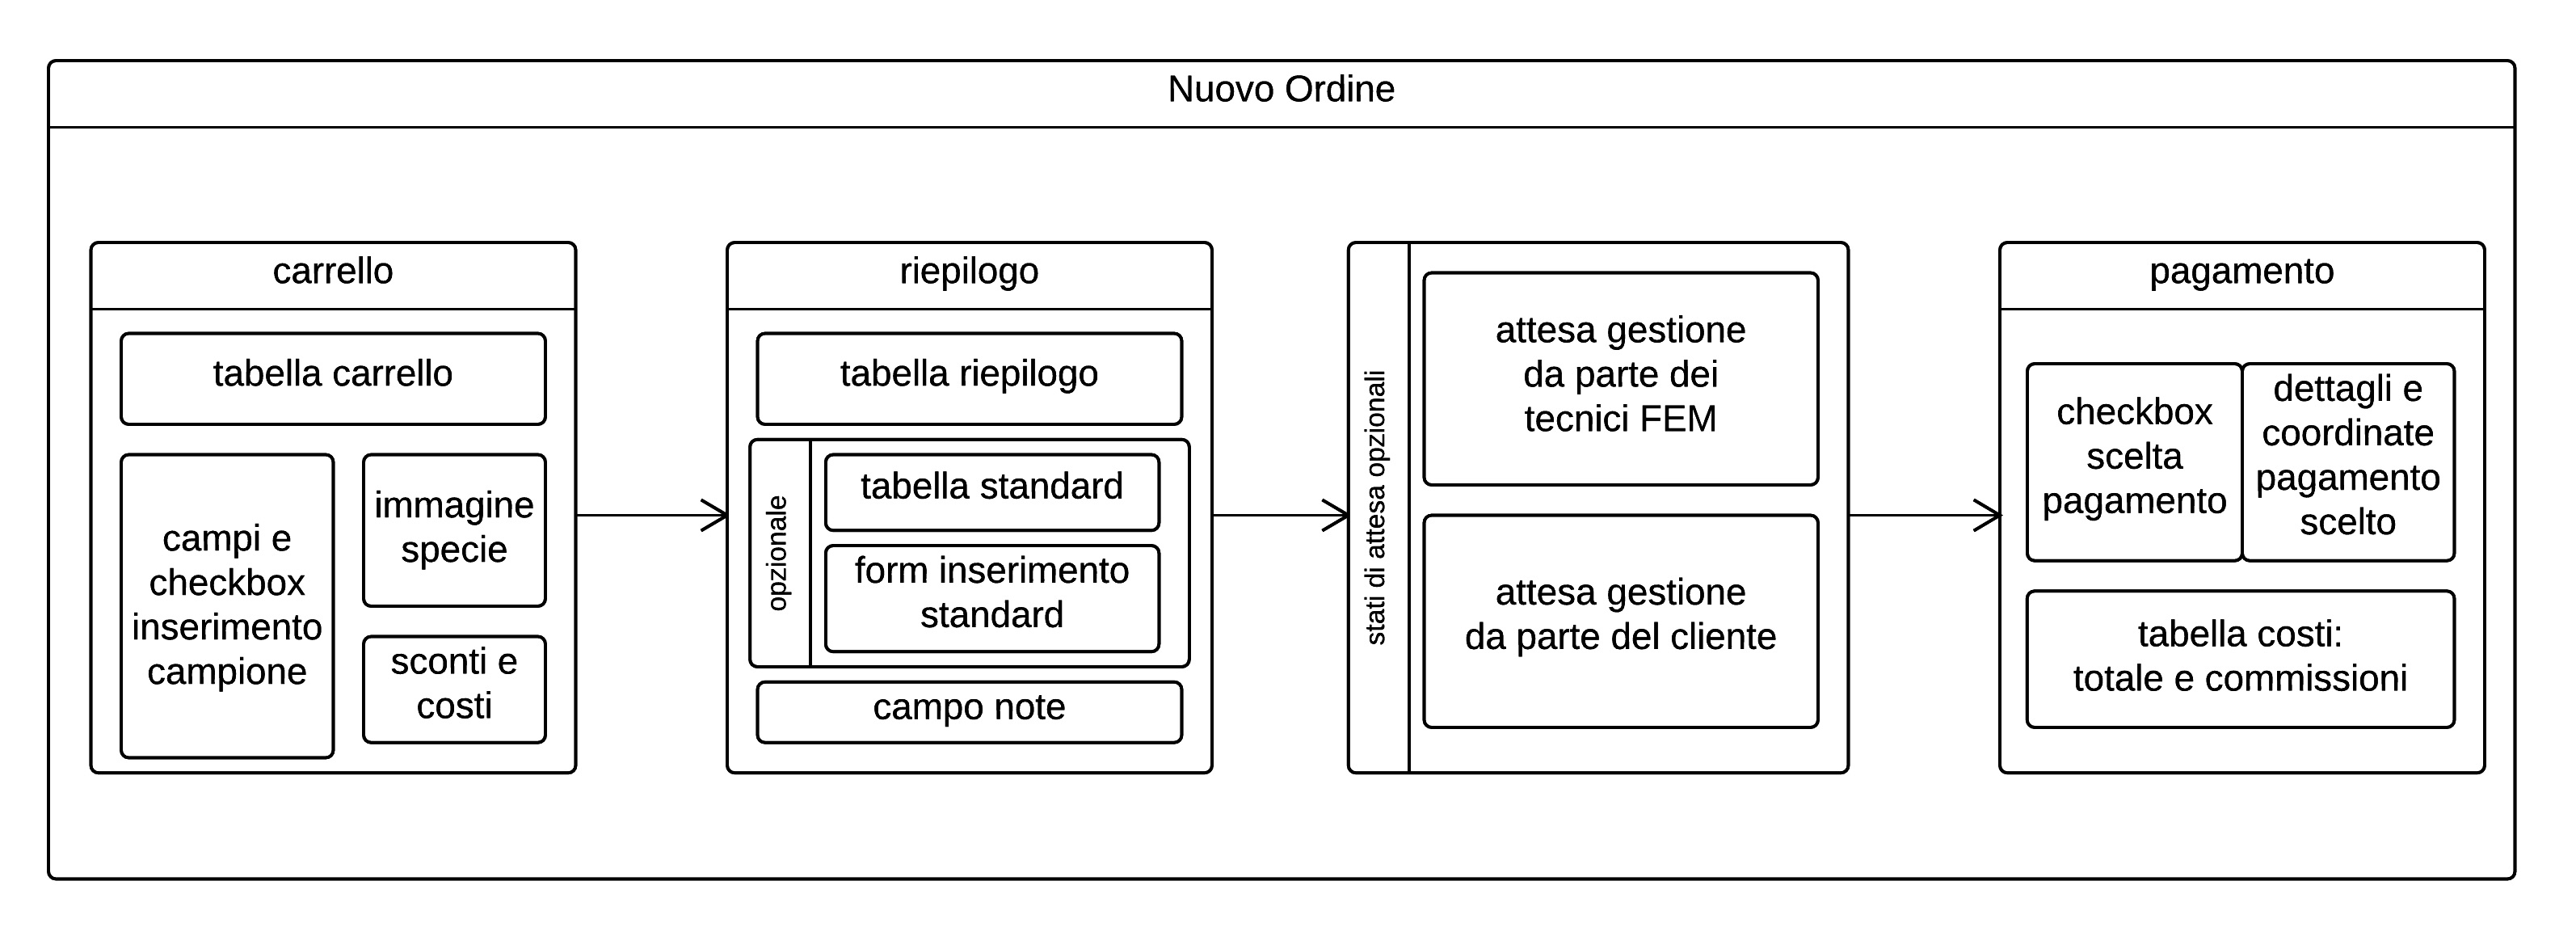
\includegraphics[width=1\textwidth]{images/nuovo-ordine-s} 
 \caption{schema della pagina per la creazione di un ordine}
 \label{fig:nuovo-ordine-s}
\end{figure}

La prima schermata del carrello a sua volta è divisa in due parti: in alto si trova la tabella che funge da carrello vero e proprio raccogliendo tutti i campioni inseriti dal cliente e mostrando i relativi dati associati come identificativo, specie, analisi richieste, costo, etc; in basso invece si trova il form per l'inserimento dei soggetti.

Come nella pagina di registrazione viene utilizzato del codice {\js} per la validazione dei campi, inoltre il campo \texttt{specie} è un elenco in cui cercare la specie e sottospecie del soggetto. 

Una volta selezionata la specie, a destra viene popolato un \tag{div} (identificato dalla classe CSS \texttt{.taxonomy}) contenente l'immagine e altre informazioni come i nomi comuni. Se non è stata correttamente selezionata la specie tra quelle esistenti il \texttt{div taxonomy} non deve comparire. Per farlo è stata creata una classe apposita in CSS (chiamata \texttt{.dno}) che imposta l'attributo di stile \texttt{display:none}, cioè oggetto non visibile, in modo tale per cui se la specie è stata selezionata correttamente vengono popolati gli appositi \tag{div} innestati contenenti il nome della specie, sottospecie, immagini e così via, al contrario in caso di errore nella selezione della specie viene aggiunta la classe \texttt{.dno} e il box \texttt{.taxonomy} non compare.

Inoltre l 'immagine potrebbe non essere presente per alcune sottospecie, in questi casi viene caricata un immagine preimpostata che lo indica al cliente.

Il seguente è un estratto del codice che si occupa del $<$\texttt{div class="taxonomy"}$>$

\begin{footnotesize}
\begin{verbatim}
if($(this).val() == "-1") {
 $(".taxonomy").addClass("dno");
} else {
 if(data_Specie[$(this).val()].immagine == "") {
  $(".image-exist").addClass("dno");
  $(".image-not-exist").removeClass("dno");
 } else {
  $(".image-exist").attr
    ("src" "/media/"+data_Specie[$(this).val()].immagine).removeClass("dno");
  $(".image-not-exist").addClass("dno");
 }
 $("#nome_specie").html(data_Specie[$(this).val()].specie_padre)
 $("#nome_sottospecie").html(data_Specie[$(this).val()].nome);
 $("#nome_comune_sottospecie").html(data_Specie[$(this).val()].nome_comune);
 $(".taxonomy").removeClass("dno");
} 
 
\end{verbatim}
\end{footnotesize}

Una volta completata l'aggiunta di soggetti si passa al \emph{riepilogo}, sezione nella quale viene riproposto l'elenco completo degli esemplari aggiunti da analizzare, e richiesta l'eventuale aggiunta di campioni standard in caso di specie classificate come junior.

Infine si visualizza la schermata per il \emph{pagamento} nella quale si sceglie attraverso un elenco di \texttt{checkbox} la modalità preferita e dinamicamente vengono descritte in un \tag{div} le coordinate per i pagamenti e per la spedizione delle piume.

Durante la creazione di un ordine può essere necessario un passo in più nel caso in cui sia stata indicata almeno una specie non presente nell'elenco fornito da {\fem}. In questo caso l'ordine viene arrestato in attesa che un addetto dell'azienda classifichi correttamente la \emph{nuova specie} indicata dal cliente. Questo avviene sia per una questione di ordine e controllo, sia per mantenere la totale correttezza al momento della generazione degli attestati ed evitare di generare documentazione con specie non esistente o scritta in modo scorretto a causa di una svista.

\subsection*{Pagina ordine}
\label{subs:po}
Completato l'ordine il cliente viene indirizzato alla pagina dedicata (figura~\ref{fig:pagina-ordine-s}) in cui vengono riproposte le coordinate di pagamento se non è ancora stato eseguito, una tabella con i soggetti da analizzare e lo spazio per le comunicazioni con {\fem}. L'elenco dei campioni permette di seguire lo stato delle analisi, vedere gli esiti e  scaricare gli attestati digitali.

\begin{figure}
 \centering
 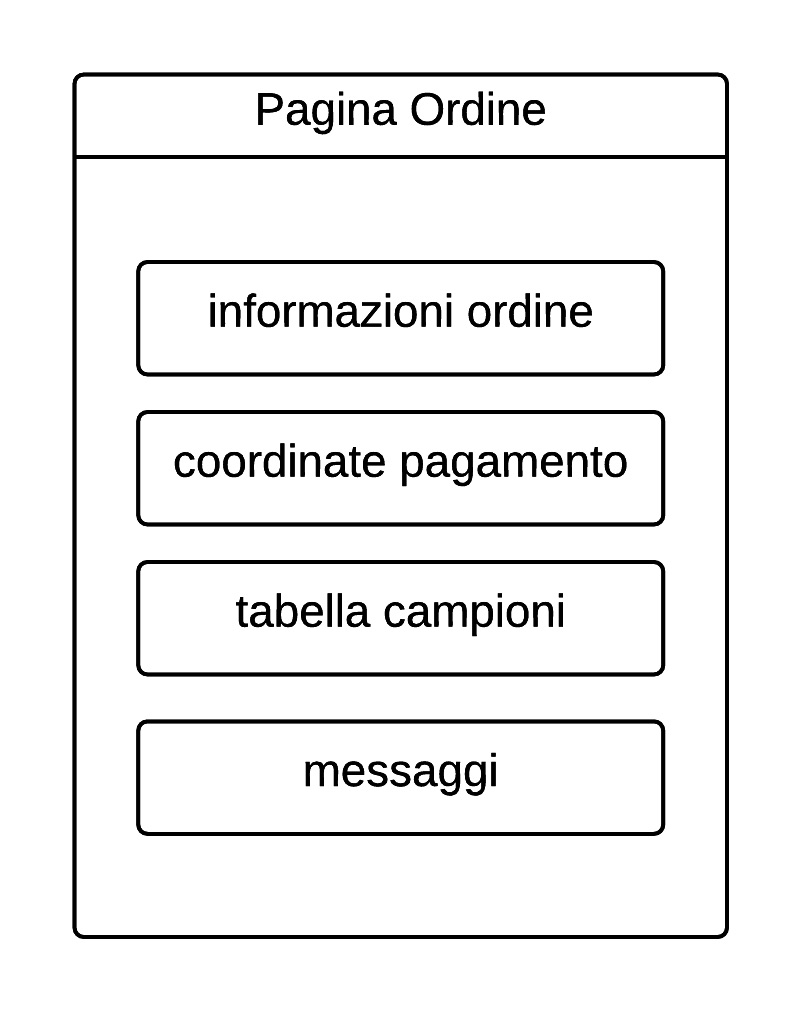
\includegraphics[width=0.32\textwidth]{images/pagina-ordine-s} 
 \caption{pagina ordine}
 \label{fig:pagina-ordine-s}
\end{figure}

\newpage
\subsection{Vista Admin}
\label{subs:admin}

%\begin{wrapfigure}{l}{0.27\textwidth}
%  \begin{center}
%    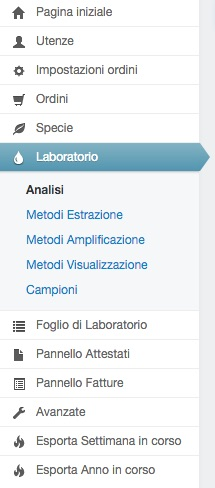
\includegraphics[width=0.25\textwidth]{images/suit}
%  \end{center}
%\end{wrapfigure}

Il controllo del flusso ordini e la comunicazione con il cliente sono una facciata importantissima per un e-commerce, e per questo motivo è necessaria una efficace interfaccia utente per la gestione di tutte le componenti da parte degli amministratori, detti admin.

Django mette a disposizione un pannello admin autogenerato basato sui modelli definiti (vedi~\ref{subs:crea}), ma per una migliore usabilità è stato installato \emph{Django Suit}, una estensione per un tema alternativo del pannello admin dei sistemi Django \cite{suit}. Django Suit ha permesso di personalizzare il lato admin andando incontro alle richieste dei tecnici di {\fem}.

La configurazione di Django Suit avviene come segue
\begin{footnotesize}
\begin{verbatim}
 SUIT_CONFIG = {
   'ADMIN_NAME': 'Pannello admin del Portale Avifauna',
   'MENU': (
     'sites',
      {'label': 'Laboratorio', 'icon':'icon-tint', 
         'models': (
            'ordini.analisi', 
            'ordini.metodoestrazione', 
            'ordini.metodoamplificazione', 
            'ordini.metodovisualizzazione', 
            'ordini.campione')},
   ),
 }
 
\end{verbatim}
\end{footnotesize}

permettendo di assegnare facilmente un titolo al pannello (\texttt{admin\_name}) e personalizzare i tasti della barra di navigazione laterale (definita \emph{menu}). Nelle righe di codice in esempio viene definito il menu dedicato al laboratorio con i collegamenti alle viste di analisi, campioni e metodi di analisi.

Gli utenti lato amministratore, cioè i dipendenti di {\fem}, si possono dividere in due tipologie: i tecnici di laboratorio e i gestori dell'e-commerce.

I primi si occupano di seguire e monitorare il corretto flusso degli ordini e delle analisi. Quando un ordine viene creato con successo compare in un apposita tabella dove è identificato dal suo numero e dal cliente che lo ha creato. All'arrivo della busta con le piume da analizzare i tecnici possono assegnare ad ogni campione un univoco identificativo di laboratorio (idlab) e, dopo aver stampato il foglio di laboratorio della giornata, effettuare le analisi. Quelle che hanno successo permettono di inserire gli esiti, generare gli attestati e far avanzare di stato l'ordine.

I gestori del sito invece hanno il compito di gestire la comunicazione e messaggistica con la clientela, oltre a monitoraggio di statistiche e iscrizioni ad associazioni.

Il dettaglio delle azioni lato admin sono descritte nell'appendice~\ref{app:admin}.
